\documentclass[tikz]{standalone}
\usepackage{chemformula}
\usetikzlibrary{shapes.arrows}
\definecolor{Gold}{rgb}{1,.844,0}
\definecolor{Silver}{rgb}{.752,.752,.752}
\begin{document}
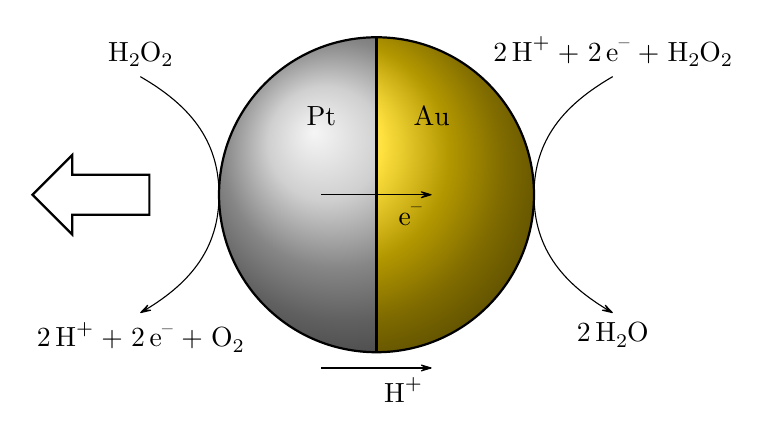
\begin{tikzpicture}[chemarrow,>=cf]
  \begin{scope}
    \clip (-2,-2) rectangle (0,2);
    \shade[ball color=Silver] (0,0) circle (2);
  \end{scope}
  \begin{scope}
    \clip (0,-2) rectangle (2,2);
    \shade[ball color=Gold] (0,0) circle (2);
  \end{scope}
  \draw[thick] (0,0) circle (2);
  \draw[thick] (0,2) -- (0,-2);
  \node at (-.7,1) {\ch{Pt}};
  \node at (+.7,1) {\ch{Au}};

  \draw[->] (-.7,0) -- (.7,0) node[below left] {\ch{e^-}};
  \draw[->] (-.7,-2.2) -- (.7,-2.2) node[below left] {\ch{H^+}};

  \node[above] at (-3,+1.5) {\ch{H2O2}};
  \node[below] at (-3,-1.5) {\ch{2 H^+ + 2 e^- + O2}};
  \draw[->] (-3,+1.5) to[out=-30,in=90] (-2,0) to[out=-90,in=30] (-3,-1.5);

  \node[above] at (3,+1.5) {\ch{2 H^+ + 2 e^- + H2O2}};
  \node[below] at (3,-1.5) {\ch{2 H2O}};
  \draw[->] (3,+1.5) to[out=-150,in=90] (2,0) to[out=-90,in=150] (3,-1.5);

  \node[draw,thick,single arrow,shape border rotate=180] at (-3.5,0) {\phantom{larrow}};
\end{tikzpicture}
\end{document}